\section{Terminologia}

La sinapsi (o giunzione sinaptica) (dal greco synàptein, vale a dire "connettere") è una struttura altamente specializzata che consente la comunicazione delle cellule del tessuto nervoso tra loro (neuroni) o con altre cellule (cellule muscolari, sensoriali). Nello specifico la sinapsi neuromuscolare rappresenta la giunzione tra neurone motore e muscolo a livello della placca motrice, ove ha luogo la trasmissione dell'impulso con le modalità delle sinapsi chimiche: lo spazio extracellulare della sinapsi neuromuscolare è detto chiave sinaptica.\cite{treccani}
La semplice associazione tra l'obiettivo di questo percorso e la parola sopra definita ha portato a denominare il middleware "Synapsis"\footnote{Traduzione in inglese del termine italiano sinapsi.}.

\subsection{Entità}

Successivamente nella trattazione verrà fatto uso del termine "entità" che, generalmente, viene intesa come insieme di elementi dotati di proprietà comuni dal punto di vista dell’applicazione considerata.\cite{treccani}
Concettualmente, in questo dominio, l'entità viene intesa come oggetto divisibile in due parti- mente e corpo- che, collegate, riescono a trasmettersi informazioni utilizzate dalla mente per raggiungere i propri obiettivi e dal corpo per diventare "attivo" nell'ambiente in cui si trova.

\subsection{Mente}

La nozione di mente può essere caratterizzata da alcuni punti chiave fondamentali:
\begin{itemize}
   \item autonomia
   \item interazione
   \item obiettivi
\end{itemize}
In altre parole, una mente può essere pensata come un componente software autonomo che interagisce con l'ambiente per svolgere i propri compiti.
I punti sopra elencati rendono facile l'associazione della mente al concetto di Agente, spiegato nella sezione \ref{jason}, poiché questa entità del Sistema Multi-Agente (MAS) ingloba astrazioni simili a quelle illustrate nella sezione \ref{jason}.

\subsection{Corpo}

Corpo è un termine generico che indica qualsiasi porzione limitata di materia, cui si attribuiscono, in fisica, le proprietà di estensione, divisibilità, impenetrabilità.\cite{treccani}
In questa trattazione è associabile alla nozione di GameObject di Unity, spiegata nella sezione \ref{unity}, utilizzata per avere una rappresentazione fisica dell'entità da realizzare.

\subsection{Azione}

Nel suo significato più generale è intesa come attività od operazione posta in essere da un determinato soggetto.\cite{treccani}
In questo studio, si considera come "azione" un certo gesto richiesto dalla mente che può essere associato ad un'operazione eseguita dal corpo, ad esempio, nel
caso di un'azione del tipo \textit{"vai a (posizione)"}, richiesta dalla mente, corrisponde il movimento del corpo nell'ambiente verso la posizione indicata.

\subsection{Percezione}

La percezione è un atto cognitivo mediato dai sensi con cui si avverte la realtà di un determinato oggetto e che implica un processo di organizzazione e interpretazione.\cite{treccani}.

\medskip

In questo studio, la percezione si collega ad una certa sensazione rilevata dal corpo ed inviata alla mente per portarla a conoscenza di questa nuova informazione, ad esempio, nel caso del raggiungimento della posizione richiesta in precedenza, il corpo trasmette la percezione \textit{"arrivato (posizione)} che informa la mente del completamento dell'operazione.

\medskip

Esiste inoltre, da parte del corpo, la possibilità di inviare percezioni "libere", ossia non associate a risposta di un'azione inviata dalla mente. Un semplice esempio è il contatto del corpo con una qualsiasi altra entità nell'ambiente che corrisponde all'invio di una percezione del tipo \textit{"toccato (nome\_entità)"}.

\subsection{Struttura entità}
Nella figura sottostante viene rappresentata la struttura di una generica entità, dove:

\begin{itemize}
   \item Il corpo esegue azioni e, in risposta a queste ultime, oppure, a seguito di determinati eventi esterni, trasmette le proprie percezioni alla mente.
   \item La mente elabora le percezioni per decidere quali azioni far svolgere al proprio corpo.
\end{itemize}

\begin{figure}[H]
   \centering
   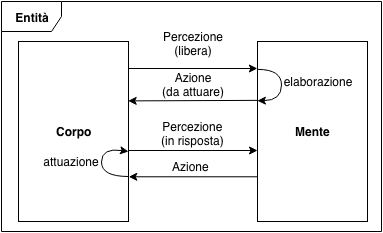
\includegraphics[width=8cm]{figures/Entita_struttura.png}
   \caption{Struttura di una generica entità}
\end{figure}
